\chapter{Frontend}

\section{Ziele}
\begin{tabularx}{\textwidth}{|l|X|}
    \toprule
    \textbf{ID-Kürzel} & \textbf{Beschreibung} \\
    \midrule
    \endhead
    \hline
    \caption{Ziele der Frontend-Architektur}
    \endfoot
    FZ-10 & Einzelne Teile des Frontends können getrennt voneinander entwickelt werden.\\
    FZ-20 & Es gibt eine Trennung von Daten- und Anzeigelogik geben.\\
    FZ-30 & Das Frontend ist leicht um neue Funktionen erweiterbar.\\
    FZ-40 & Das Frontend ist responsiv gestaltet.\\
\end{tabularx}

\section{Views}
Da die Anwendung auf mehreren Plattformen laufen soll wird die Applikation als HTML5 App programmiert.
Dabei besteht das Frontend aus folgenden Views:
\begin{tabularx}{\textwidth}{|l|X|l|}
    \toprule
    \textbf{ID-Kürzel} & \textbf{Beschreibung} & \textbf{Route}\\
    \midrule
    \endhead
    \hline
    \caption{Einsatzbereiche}
    \label{Einsatzbereiche:tabelle}
    \endfoot
    F-10 & Newsfeed & \verb+/+\\
    F-20 & User Login & \verb+/login+ \\
    F-30 & User Registrieren & \verb+/register+ \\
    F-40 & Profilverwaltung und Einstellungen & \verb+/profile+\\
    F-50 & Detailansicht von Einträgen & \verb+/+\\
    F-60 & Adminansicht & \verb+/administration+\\
\end{tabularx}

\section{Newsfeed}
Der Newsfeed ist eine Kollektion aus Einträgen und Vorschlägen (Informationen). Diese werden nach Relevanz sortiert.
Dabei kann das Frontend die Einträge abfragen. Der Server ist verantwortlich für die Sortierung der Einträge.

\subsection{Bearbeiten des Newsfeeds}
\begin{figure}[H]
    \centering
    \includegraphics[width=0.9\textwidth]{images/DialogeFrontend.png}
    \caption{Ablauf von Dialogen}
\end{figure}

Ein Benutzer muss sich immer Authentifizieren bevor er seinen Newsfeed sieht.
Anschließend erhält er eine Übersicht seiner Einträge. Jetzt hat er die Möglichkeit Einträge anzulegen, verändern, löschen oder einen
Vorschlag in seinen Newsfeed aufzunehmen.
Wenn ein Eintrag erstellt oder bearbeitet wird öffnet sich ein Dialog in dem der entsprechende Eintrag bearbeitet werden kann.
Anschließend wird der neue Newsfeed dargestellt.

\section{Profilverwaltung und Einstellungen}
In der Profilverwaltung und den Einstellungen  kann der Benutzer sein Passwort, Username oder E-Mail ändern. 
Außerdem kann eingestellt werden, ob der Benutzer an Einträge erinnert werden möchte oder nicht (Notifikationen).



\section{Komponenten der Anwendung}
\begin{figure}[H]\label{frontend:mockup}
    \centering
    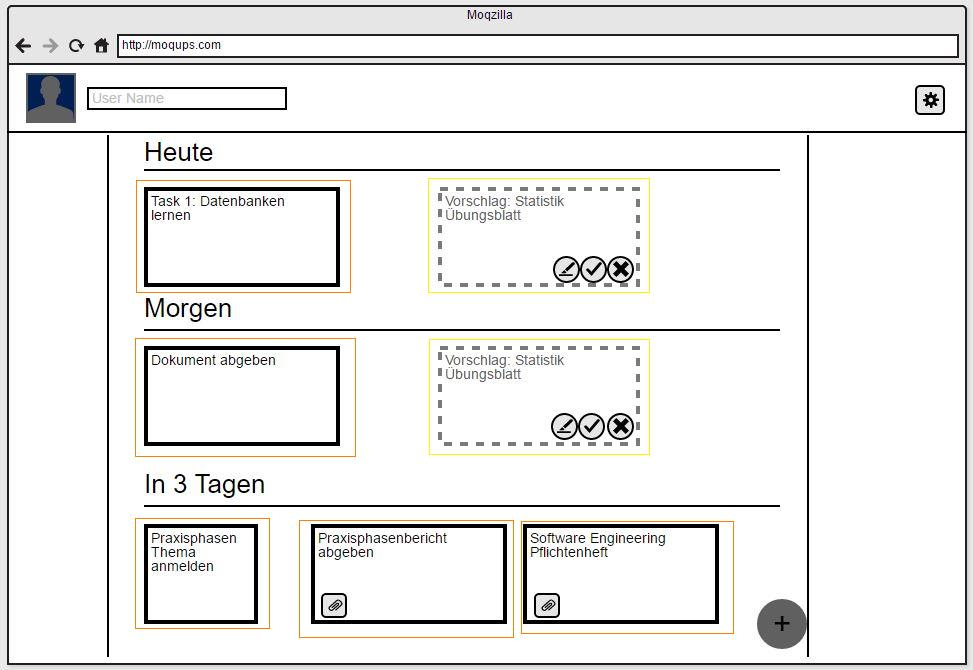
\includegraphics[width=0.7\textwidth]{images/mock-up.JPG}
    \caption{Komponenten des Newsfeeds}
\end{figure}

Wie in Abbildung \ref{frontend:mockup} zu sehen ist besteht die Anwendung aus mehreren Einträgen und Vorschlägen.
Diese UI-Elemente können als Komponenten angesehen werden.  
Deshalb soll das UI auf React.js basieren, da dort jedes UI-Element eine Komponente ist, die einen Zustand hat und mehrere Aktionen ausführen kann.
Der Zustand beinhaltet immer die anzuzeigenden Daten. Wird eine Aktion wie z.B. ein Klick-Event ausgelöst ändert sich der Zustand und die Komponente wird
neu gerendert.\footnote{Siehe \url{https://facebook.github.io/react/}}
Dies erleichtert die Entwicklung der Anwendung im Team und erhöht die Wiederverwendung von UI-Komponenten.

\section{Trennung von Daten und Anzeigelogik}
Eines der Ziele ist es Daten und Anzeigelogik getrennt von einander zu entwickeln. 
Deshalb können nicht alle Daten in den UI-Komponenten gespeichert werden. Möchten z.B. mehrere Komponenten auf die selben 
Daten zugreifen wird ein extra Lager (Store) für diese Daten benötigt.

Dazu wird Flux als ein Architektur Pattern eingesetzt.
Die Grundbestandteile dieser Architektur sind Komponenten, Storages, Actions und ein Dispatcher.
Dabei dienen die Komponenten zur Interaktion mit dem User, stellen somit also den \enquote{View} der Anwendung dar.
Die Komponenten können Actions auslösen, welche einfache Funktionen sind die ausgeführt werden.
Diese Actions senden ein Objekt mit einer ID an den Dispatcher, welcher die Objekte an alle Stores verteilt.
Ein Store ist wie der Name schon sagt ein Ort zum lagern von Daten. Jeder Store stellt eine Methode \enquote{handleAction} zur Verfügung.
Diese wird von dem Dispatcher aufgerufen und das Objekt der Action übergeben. 
Anschließend kann der Store aufgrund der in der Action definierten ID seine Daten aktualisieren.
Jetzt können sich Komponenten bei dem Store registrieren um über Änderungen informiert zu werden.
Geschieht dies wird der View der Komponente erneuert. \footnote{Vgl. \url{https://facebook.github.io/flux/}}
\begin{figure}[H]
    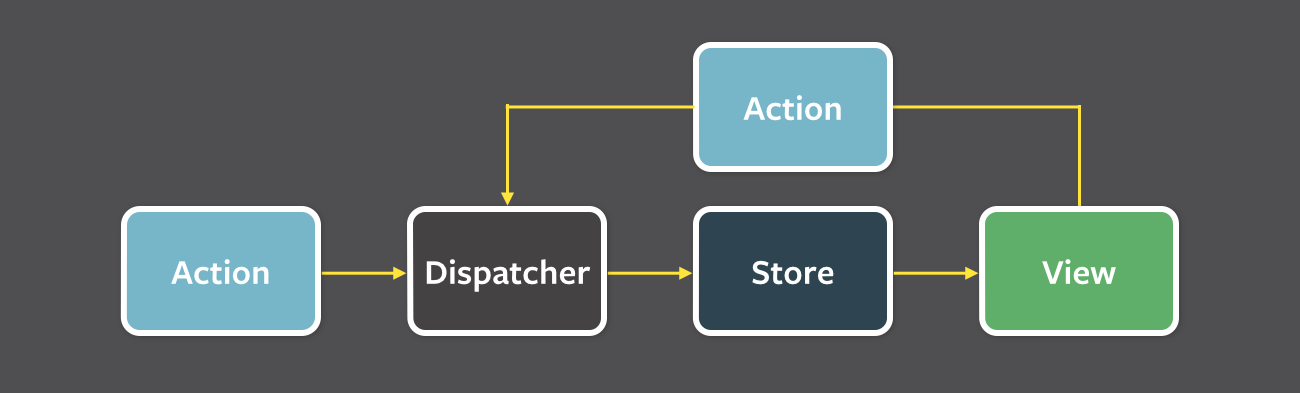
\includegraphics[width=\textwidth]{images/flux.png}
    \caption{Flux}
    \url{https://facebook.github.io/flux/docs/actions-and-the-dispatcher.html#content}
\end{figure}

Diese Architektur unterstützt das Teilen eines Zustandes mehrerer Komponenten, da sich mehrere Komponenten auf einen Storage registrieren 
und Änderungen an dem Zustand der Anwendung immer global über eine Action ausgeführt werden. Somit können alle Stores ihre Daten bei spezifischen Aktionen aktualisieren.
Dadurch wird vermieden, dass sobald sich ein Eintrag ändert eine extra Methode geschrieben werden muss welche den Newsfeed ändert.

